%
% include the class file for USI-INF Technical Reports
%
\documentclass{usiinftr}
\usepackage{float}
\usepackage{amsmath}
\usepackage{slashbox}
\usepackage{subfigure}

%
% if you want to create a cover page only (e.g. to put it in front
% of a WORD document or the like), use the "coverpage" option
%
%\documentclass[coverpage]{usiinftr}

%%%%%%%%%%%%%%%%%%%%%%%%%%%%%%%%%%%%%%%%%%%%%%%%%%%%%%%%%%%%%%%%%%%%

\begin{document}

\title{Adapting \texttt{cuda\_launch\_config} compute grid configurator for multidimensional plain and compiler-generated\\ GPU kernels}

%\author{Lawrence Farinola}{1}
\author{Zdenek Pesek}{1,2}

\affiliation{1}{\USIINF}
\affiliation{2}{Faculty of Information Technology, Czech Technical University in Prague}

%
% put the number of your Technical Report here; in order to determine
% the number, take the number of the most recent USI INF Technical Report
% (on top of the list at http://www.inf.usi.ch/techreports/) and increment
% it by one; the format is "[year]-[number]"
%
\TRnumber{2014-2}

%
% by default, the current month and year are used as the publication date
% of your Technical Report; if you want to change this, then you can do it here, e.g.
%
%\date{February~\the\year}
%\date{August 2011}

\maketitle

\begin{abstract}

Exploiting the potential of GPU computing is inevitable for any modern HPC application. One of the crucial aspects of programming efficient CUDA kernels is choosing the optimal compute grid/block configuration. Hard-coded configuration of block size (e.g. \{128, 1, 1\}) is known to give good performance results on Fermi and Kepler GPUs, however faster configuration could potentially be found for each individual kernel, if its specific properties are accounted.
\vskip4pt
Our work is based on \texttt{cuda\_launch\_config} -- an existing framework for heuristic search of semi-optimal grid/block configuration, originally designed for 1-dimensional Thrust kernels. We modified it to determine optimal setups for multidimensional kernels and added an interface layer to use it inside KernelGen GPU auto-parallelizing compiler. These contributions allowed us to improve the performance of GPU kernels of stencil benchmark by up to XX\% in case of manually-written CUDA code and by up to 7\% for kernels generated by KerenGen compiler.

\end{abstract}

\section{Introduction}

Possible points to cover in introduction:

\begin{itemize}
\item The problem of compute grid selection is a major obstacle in understanding CUDA by n00bs
\item The concept of occupancy is often discussed in overcomplicated way
\item Paper structure
\item \texttt{cuda\_launch\_config} is designed for Thrust, and this uses only 1D blocks.
\end{itemize}

The paper is organized as follows. Section \ref{sec:compute_grid} explains the key factors of optimal CUDA compute grid choice.

\section{Choosing efficient compute grid}
\label{sec:compute_grid}

Possible points to cover in this section:

\begin{itemize}
\item Key CUDA kernel \emph{code} characteristics: regcount, shared memory
\item How regcount and shared memory could become kernel performance limiters (examples)
\item What else could be kernel performance limiters
\item How to account all limitations together
\item cuda\_launch\_config's approach
\end{itemize}


\section{Implementation for autoparallelizing compiler runtime}

\begin{itemize}
\item Making cuda\_launch\_config to play together with runtime constants substitution
\end{itemize}

\section{Benchmarking}

For benchmarking was used the integrated set of tests in KernelGen, which was executed on the Tesla-CMC cluster with {NVIDIA} Tesla C2075 graphic cards. Execution of the performance tests was handled by the KernelGen script called Buran.

Because of the KernelGen limitations, it was not possible to execute all the need CUDA functions in the cuda\_launch\_config library. Thus, required parameters had to be supplied externally from the caller function in KernelGen. Almost all these attributes were already present in the code, so they were just passed to the library. The only exception was a maximal threads per block value, which had to be determined heuristically. Consecutive benchmarking showed us, that selection of this value is crucial for the whole algorithm and performance respectively.

\subsection{First version}

For the first version, the value of threads per block was computed as a closest power of two. When looking at the result chart \ref{fig:clc1} , it was not the best idea and definitely some more tuning needed to be done. There is a speedup of a 10\% in one of the test cases, but the overall result is worse than the origanl version and this is not acceptable if we want to use this version in the real world. However, this initial step gives us a good entry point to start with.

\begin{figure}[H]
\begin{center}
  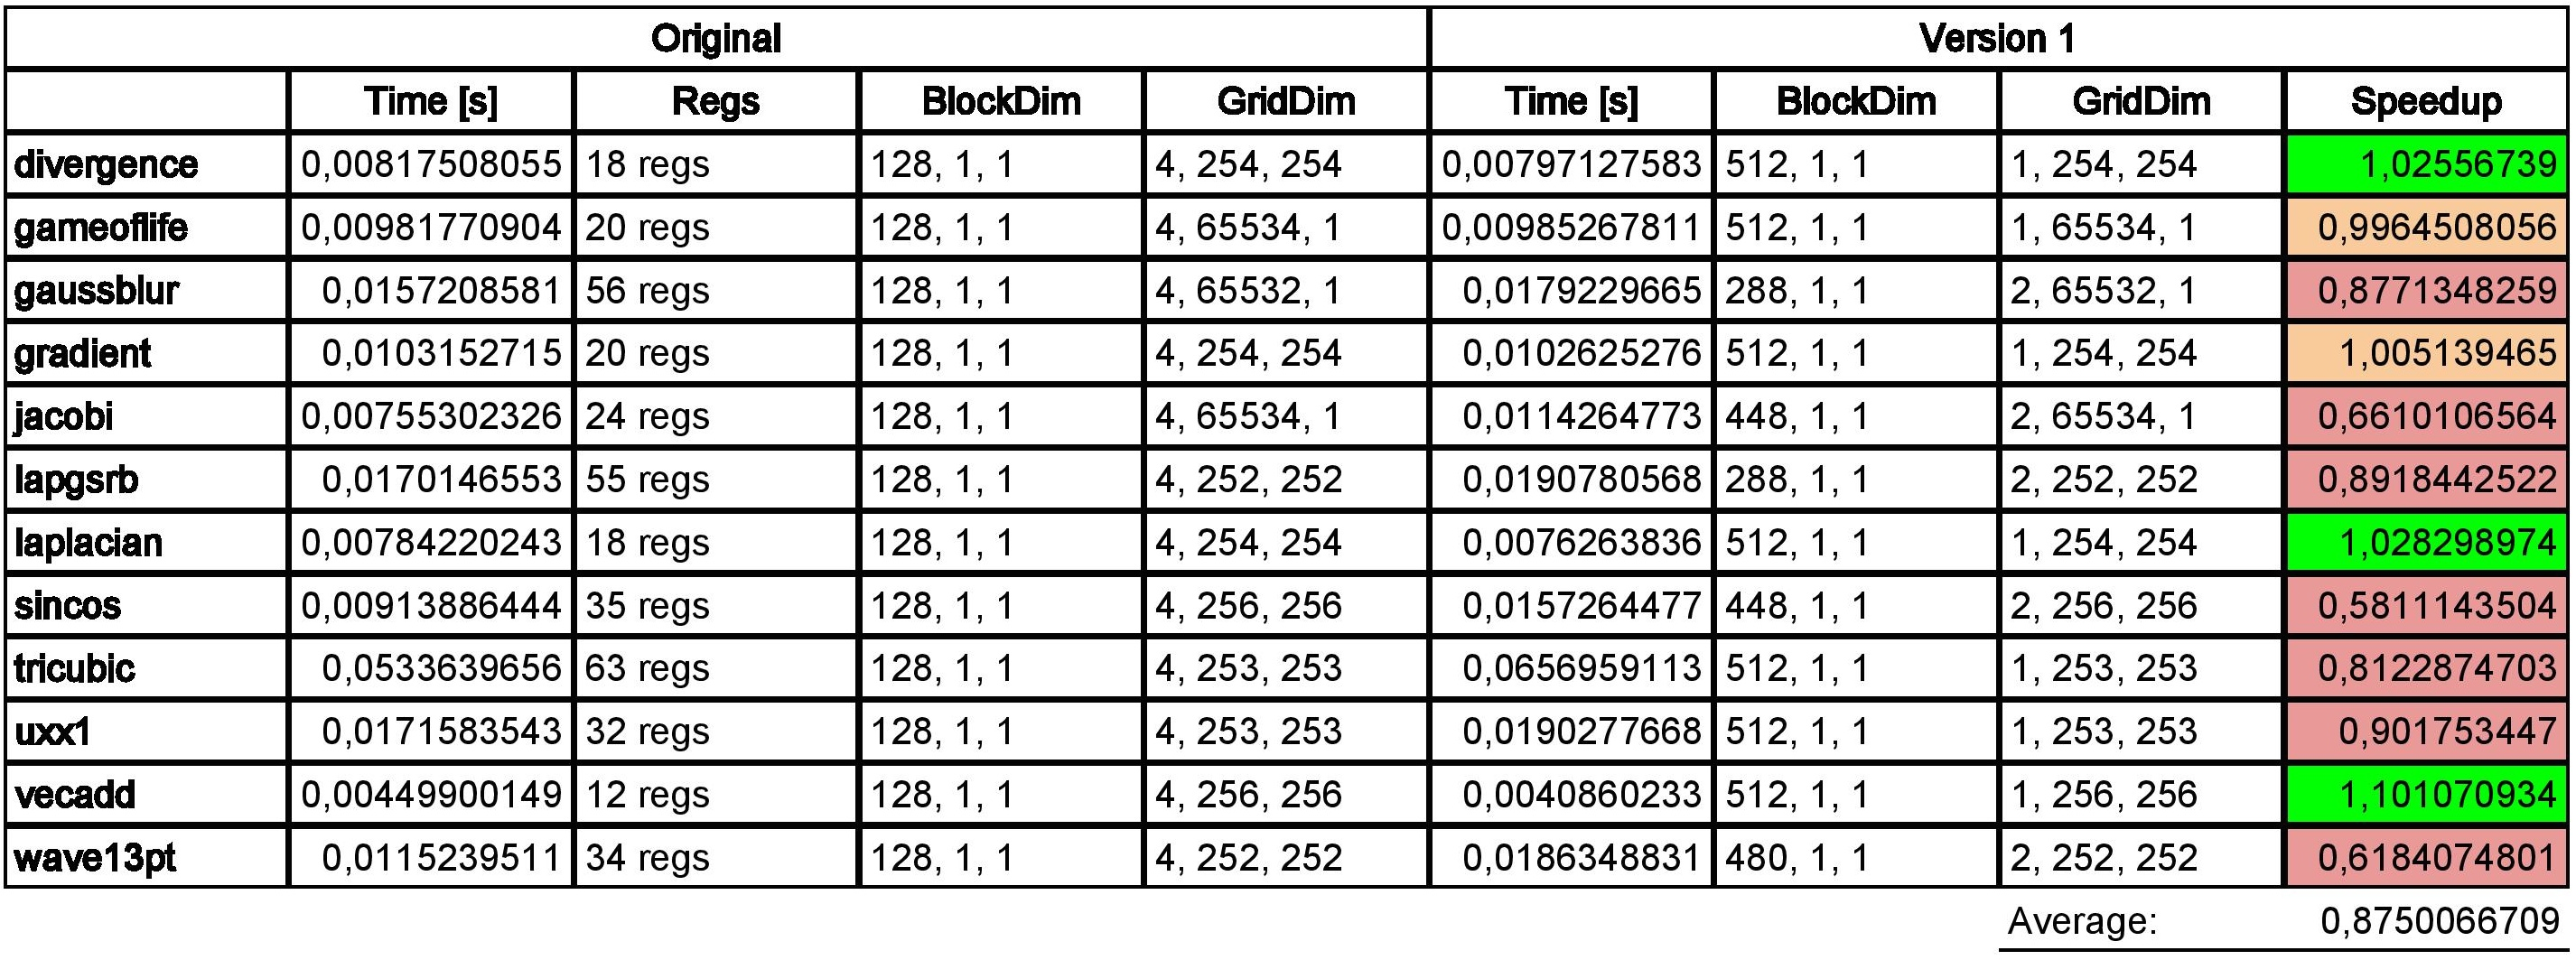
\includegraphics[width=1\textwidth]{figures/kernelgen_v1}
  \caption{Comparsion of the original KernelGen results and the first version with cuda\_launch\_config  \label{fig:clc1}}  
\end{center}
\end{figure}

\subsection{Second version}

The second version showed \ref{fig:clc2} the impact, a correct selection of a block grid can have. The limiting factor was now calculated as a nearest power of two lower than the the input value. There are signifacnt differences in speedup when compared to the first version. But, deviations from the normal can be seen in both ways. Especially in the sincos benchmark, the result is very bad. Assuming, that the original hard-coded value 128 was a good estimation of an average value, the resulting block grid is still to big. The overall performance is now almost equal to the original version, but we want to see there a number clearly higher than one. Also, results of the test cases should be more consistent - ideally same or better than the original version for majority of test cases.

\begin{figure}[H]
\begin{center}
  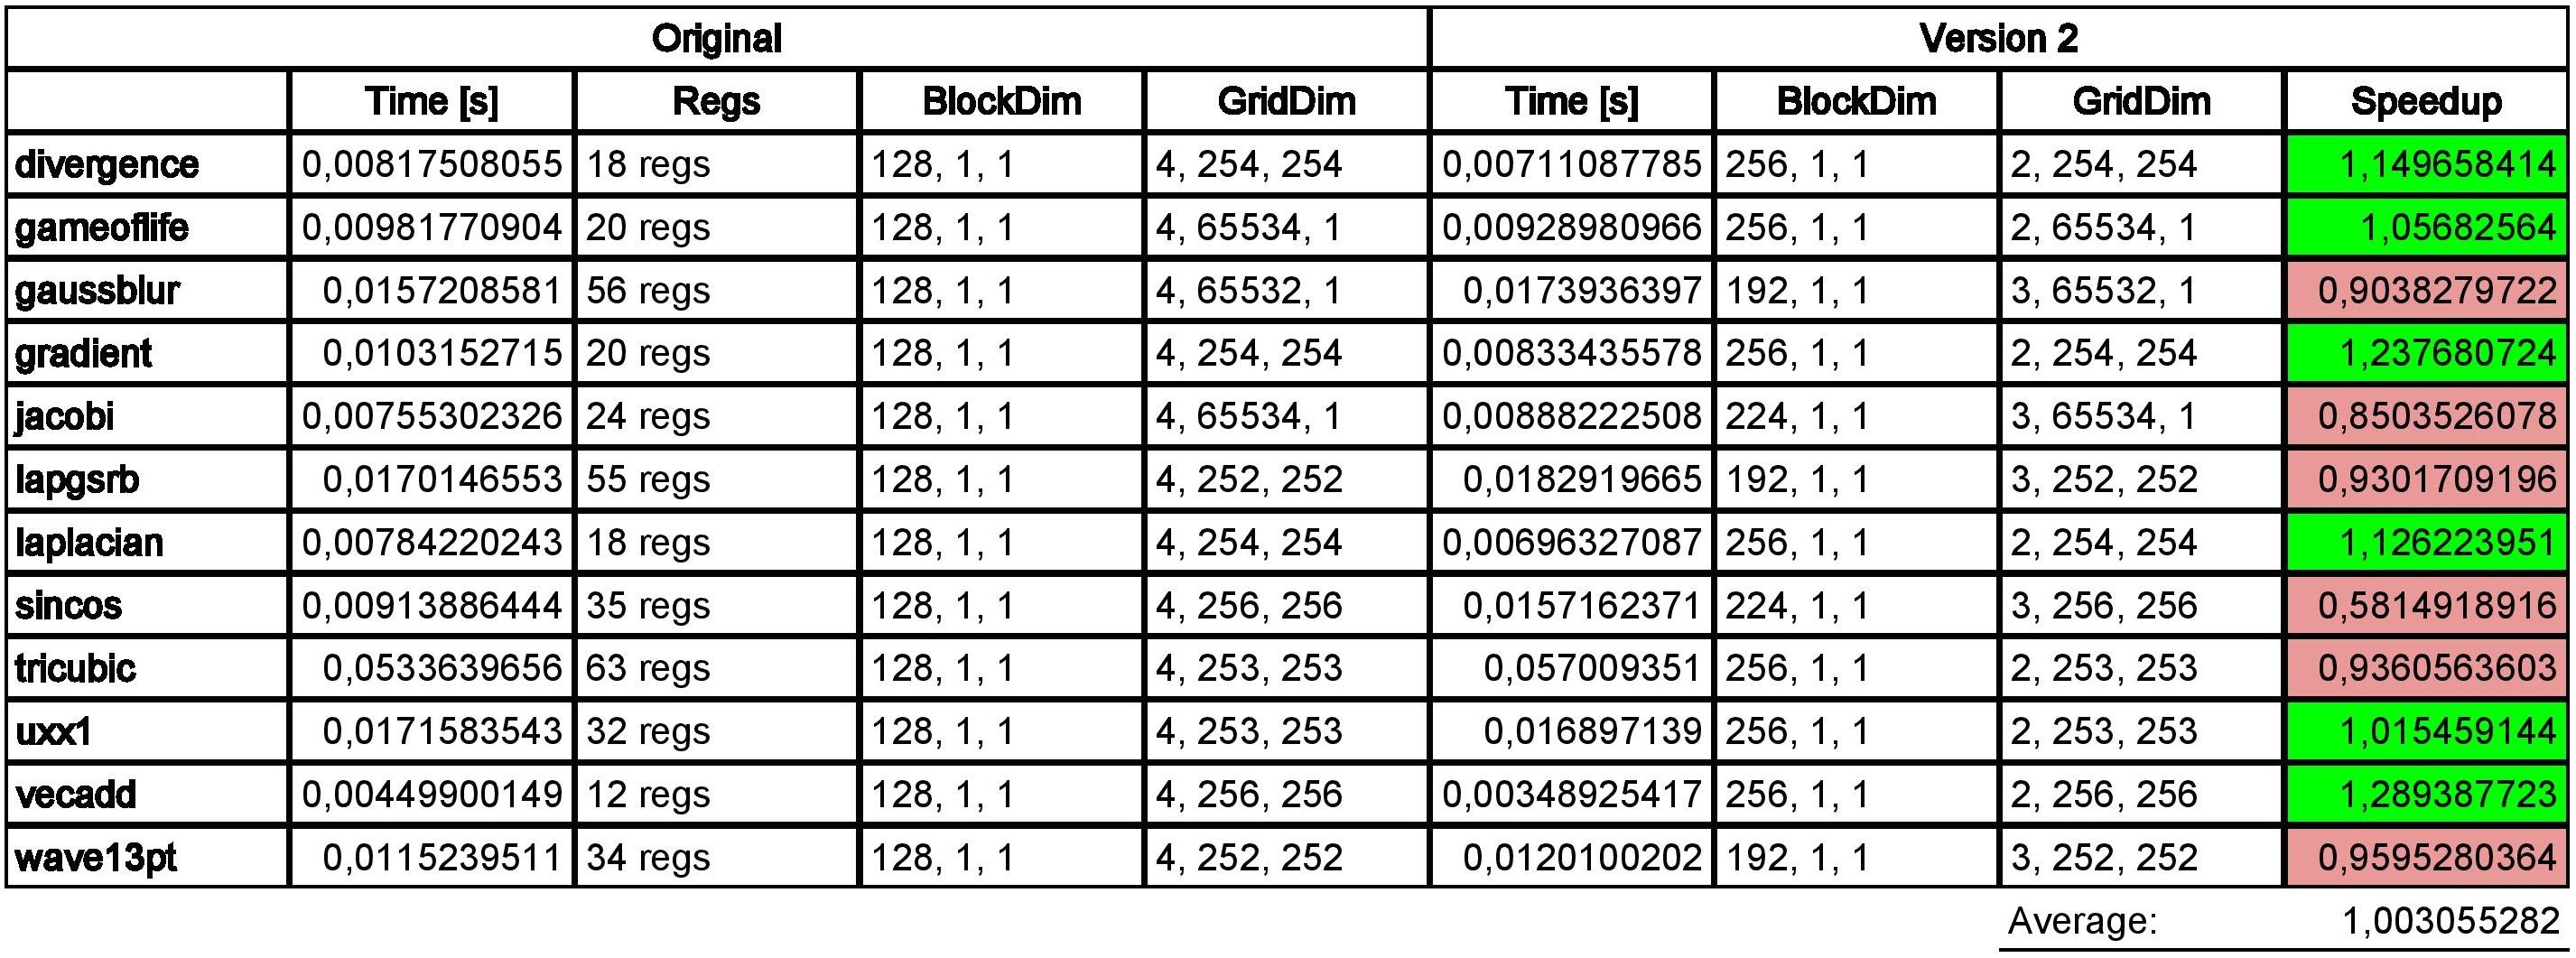
\includegraphics[width=1\textwidth]{figures/kernelgen_v2}
  \caption{Comparsion of the original KernelGen results and the second version with cuda\_launch\_config \label{fig:clc2}}  
\end{center}
\end{figure}

\subsection{Third version}

The third and final version performed really well \ref{fig:clc3}. It produced the best results, which could be suitable for the production version use. Requirements stated when commenting the previous chart were met in this case. Speedup values are now more consistent. Appart from a single performance test, all generated block configurations are resulting in the same or even better performance than in the original version. A key to this final step was lowering the maximal threads per threads per block value by one additional shift right operation. For the first time, we can see even lower number of threads in the block grid than the original 128. Both tests with the block grid set to 96 are significantly faster than before. The final average improvement is almost 7\%.

\begin{figure}[H]
\begin{center}
  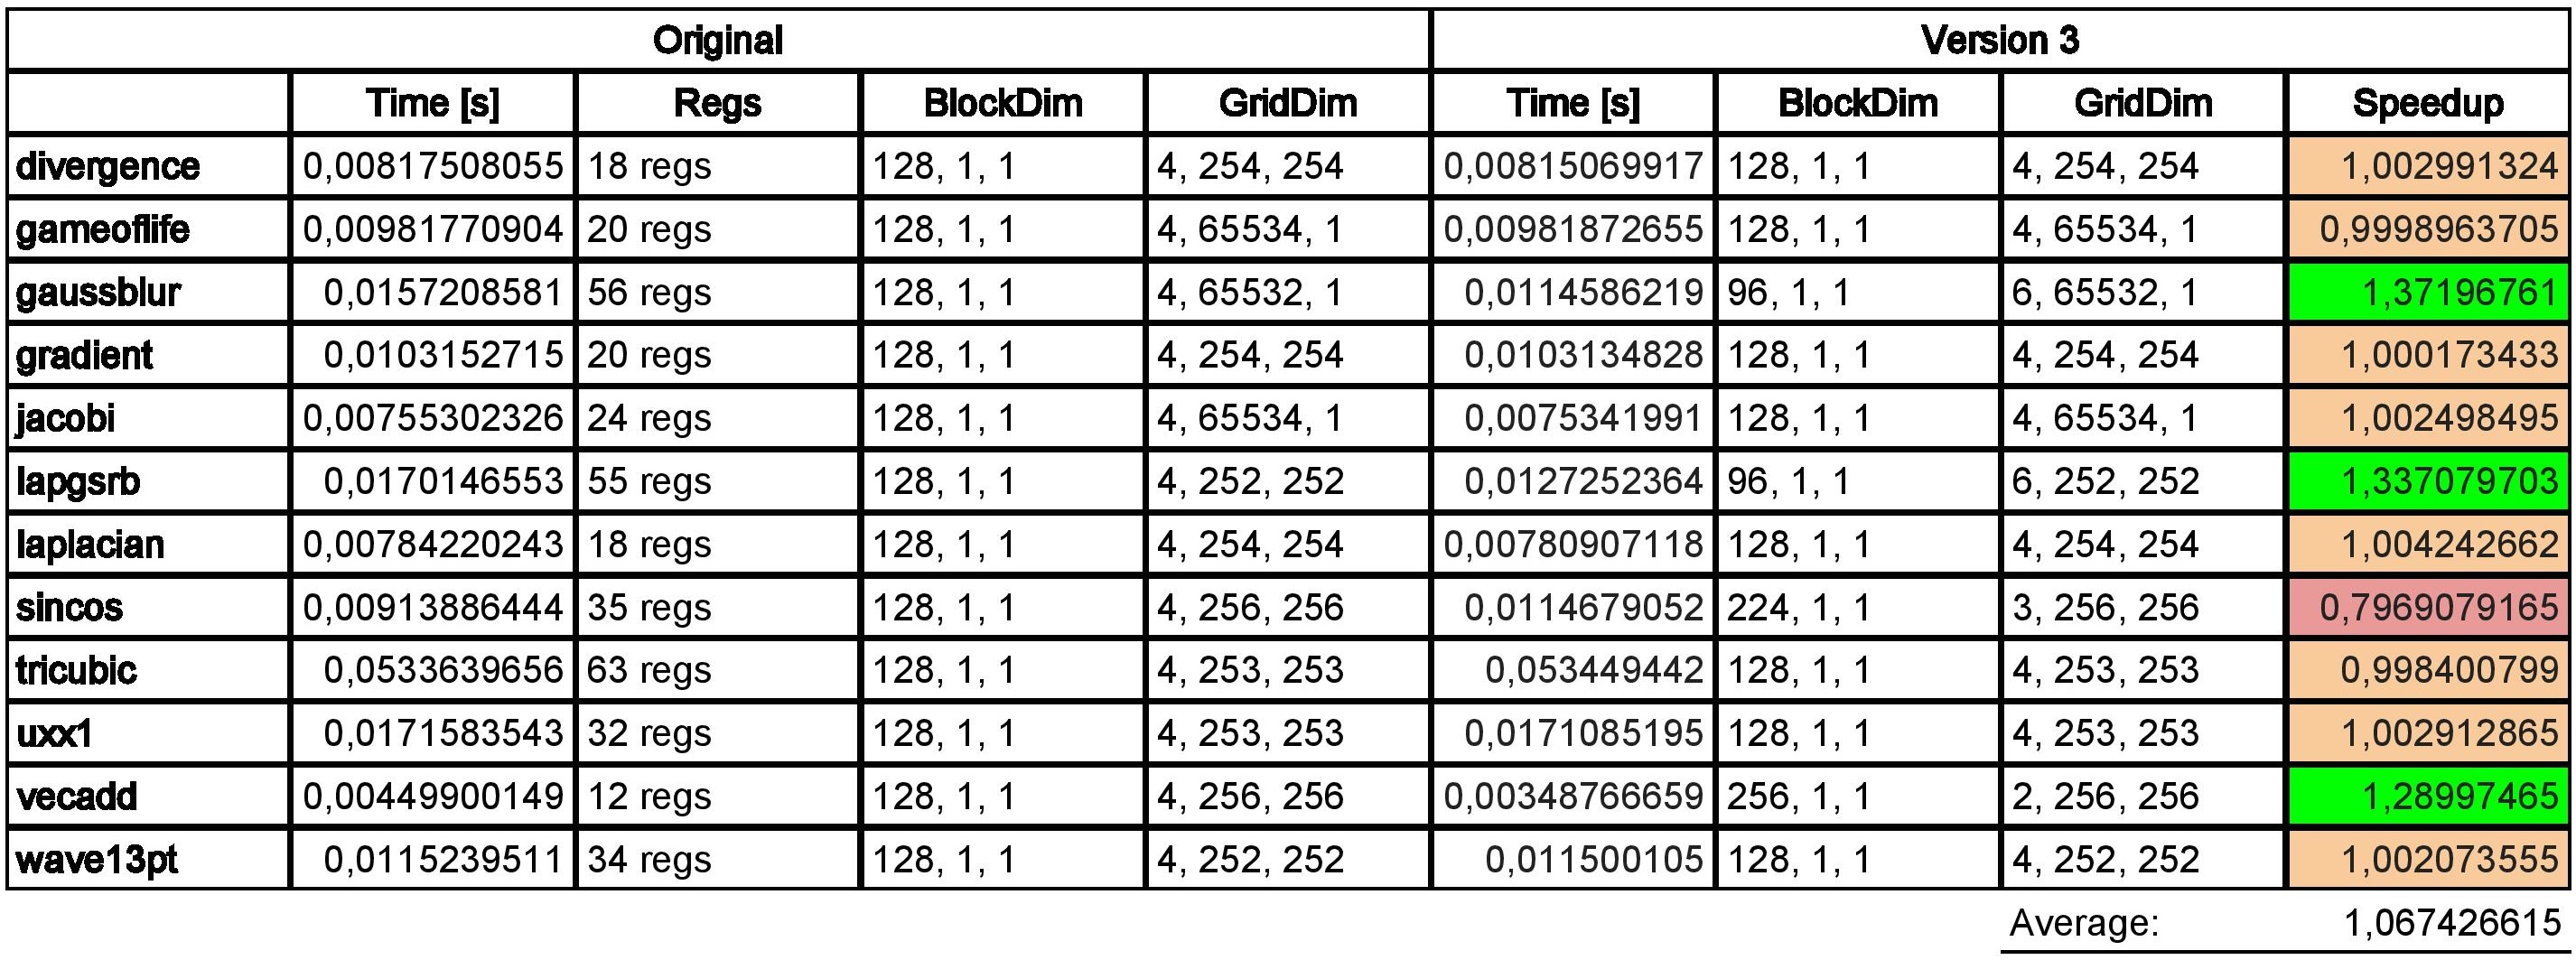
\includegraphics[width=1\textwidth]{figures/kernelgen_v3}
  \caption{Comparsion of the original KernelGen results and the third version with cuda\_launch\_config \label{fig:clc3}}  
\end{center}
\end{figure}

\section{Conclusion} 

To summarize this report we need to look back at the beginning, where the important question was stated - Can be cuda\_launch\_config project library successfully used for a large-scale kernel configuration generation? According to the benchmarking results, automatic block grid generation was the right step forward. It also proved, that the occupancy metric was selected correctly to evaluate theoretical kernel performance and has a great impact on the final result. Two of the three speedups were achieved with a block size of 96 threads, which is even lower value than the original 128 threads. These two kernels are using a lot of registers on the GPU, which are strictly limited. This means, that only few kernels can be assigned to one SM at the same time. Thus, in order to achieve higher occupancy and to be able to assign more kernels to a single SM, we have to decrease the number of threads per block. Average speedup improvement of almost 7\% is a very promising result and together with this paper represents a solid base for the possible future work. It would be interesting to investigate the iterative approach used for grid generation.

\emph{Acknowledgements (if any) ...}

\section{Related work}

\begin{itemize}
\item CUDA occupancy calculator
\end{itemize}

Google for topic and add related studies, if there are any.

\bibliographystyle{plain}
\bibliography{citations}

\end{document}